\documentclass[10pt,handout]{beamer}

\usepackage[french]{babel}
\usepackage[T1]{fontenc}
\usepackage[utf8]{inputenc}
\usepackage[
    left = \flqq{},%
    right = \frqq{},%
    leftsub = \flq{},%
    rightsub = \frq{} %
]{dirtytalk} 	% for \say{}
\usepackage{xcolor} 	% for color text
\usepackage{csquotes}
\usepackage{amssymb}
\usepackage{mathtools}
\usepackage{array}

\usetheme{Frankfurt}
\usetheme{CambridgeUS}
\usetheme{JuanLesPins}
%\usetheme{Montpellier}
%\usetheme{Madrid}

\usecolortheme{dolphin}

\useinnertheme{circles}
\usefonttheme{structurebold}
\useoutertheme{default}

%\hypersetup{pdfpagemode=FullScreen}

\title[Chemins spécifiques]{Chemins spécifiques pour la classification dans les réseaux de neurones profonds}
\author[Bouzidi, Elhouiti, Kezzoul, Zeroual, Dadi]{Bouzidi Belkacem - Dadi Mélissa \\ Elhouiti Chakib - Kezzoul Massili \\ Zeroual Ramzi}
\institute[]{Université de Montpellier}
\date{\today}

% Pour inserer une frame de sommaire avant chaque debut de section
\AtBeginSection[]
{
  \placelogofalse
  \begin{frame}
    \tableofcontents[hideothersubsections,currentsection,subsectionstyle=show/shaded/hide]
  \end{frame}
  \placelogotrue
}

% Mettre les listes en triangle
\setbeamertemplate{itemize item}[triangle]

%Insertion d'un logo
\newif\ifplacelogo % create a new conditional
\placelogotrue % set it to true
\logo{\ifplacelogo
\includegraphics[height=12mm]{img/univ-montpellier.png}\fi}

%------------------------------------------------------%
% page de titre
%------------------------------------------------------%
\begin{document}

\placelogofalse
\begin{frame}
	\titlepage
\end{frame}

\placelogotrue

\section{Introduction}
\subsection{Les réseaux de neurones profonds}

\placelogofalse 
\subsection{Le jeu de données}
\begin{frame}{MNIST}
    \makebox[\textwidth]{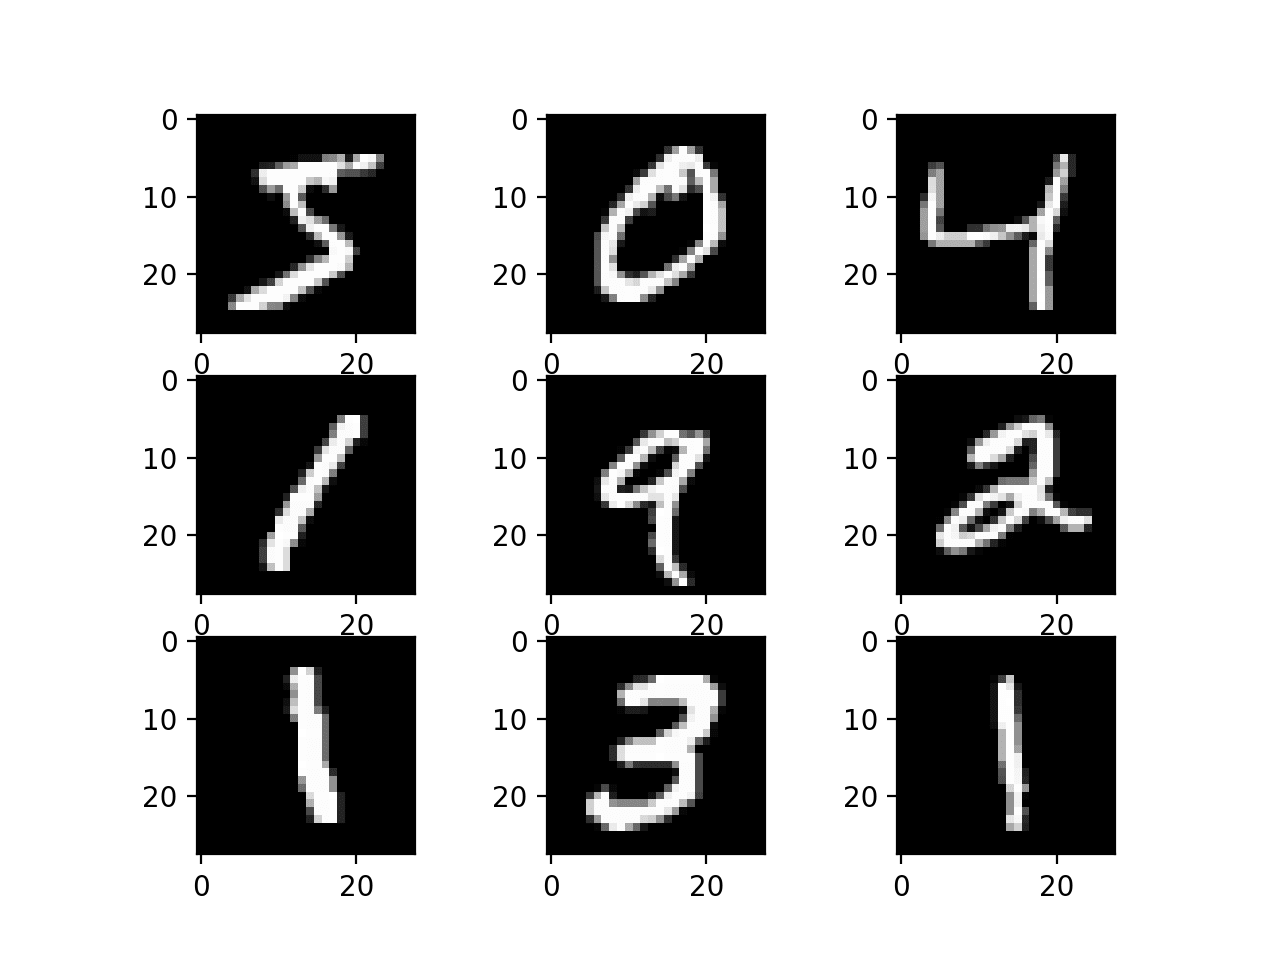
\includegraphics[width=0.8\textwidth]{img/mnist.png}}
\end{frame}
\placelogotrue

\placelogofalse 
\subsection{Problèmatique}
\begin{frame}{Problèmatique}
    \begin{block}{Boite noire}
        Les réseaux de neurones semblent s'appliquent à la manière d'une boite noire. Aucune information n'est fournie sur ce qui les a conduits à atteindre leurs prédictions.
    \end{block}
    \begin{block}{Objectifs}
        L'objectif est de comprendre le fonctionnement interne d'un réseau de neurones et de repérer des signatures d'activation de neurones en variant les données.
    \end{block}

    \makebox[\textwidth]{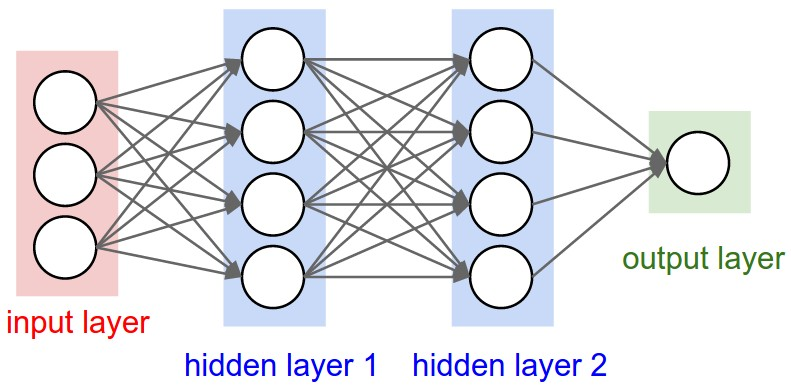
\includegraphics[width=0.6\textwidth]{img/ann-dense.jpg}}
        
\end{frame}
\placelogotrue

\begin{frame}{Questions qu'on se posent}
    Par exemple, si on entraîne un modèle à reconnaître des images de 1 et de 7
    \begin{itemize}
        \item À partir de quelle couche le modèle change de comportement pour reconnaître une image ?
        \item Les signatures des images de \textit{7}, sont-elles différentes de ceux des \textit{1} ?
        \item Si on passe une image de \textit{3} au modèle, à quoi va ressembler sa signature ?
    \end{itemize}    
\end{frame}

\subsection{Solution proposée}
\begin{frame}{Solution proposée}
    \begin{itemize}
        \item Construire des réseaux de neurones.
        \item Récupérer, pour chaque donnée, la sortie des couches cachées.
        \item Extraire les signatures grâce à des algorithmes de \textit{clustering}.
        \item Réaliser une interface de visualisation en utilisant différentes techniques.
        \item Analyser les résultats et répondre aux questions.
    \end{itemize}
\end{frame}

\section{Organisation}

\section{Analyse des données}
\begin{frame}
    \begin{block}{Importance de l'analyse}
        L'objectif de l'analyse des données, c'est de savoir comment sont nos données et comment on peut les utiliser.
    \end{block}
\end{frame}


\subsection{Découpage des données}

\begin{frame}{Découpage des données}
    \begin{itemize}
        \item Garder un nombre précis d’images pour un ensemble de chiffres définis.
        \item Faciliter la phase de développement.
        \item Pouvoir mieux visualiser les résultats sur un petit
        ensemble de données.
    \end{itemize}
\end{frame}

\subsection{Prétraitement}
\begin{block}{Scaling}
    Utilisation de la normalisation, qui consiste à
    mettre les valeurs des images entre 0 et 1 au lieu de 0 et 255.
\end{block}
\begin{block}{Flattening}
    Aplatissement des images pour avoir un tableau à une seule dimension au lieu d’une matrice à deux dimensions.
\end{block}
\begin{block}{}
    Transformation des labels en un vecteur binaire contenant que des 0 et des 1.
    \begin{itemize}
        \item Taille du vecteur égale au nombre de labels uniques à garder.
        \item Tri des labels à garder.
        \item Mettre un 1 à la case du label correspendant
        et des 0 aux autres cases.
        \item Ex: transformation en vecteur des images de 1, 3 et 7.
        \item Pour un 1 $\implies$ [1,0,0].
        \item Pour un 3 $\implies$ [0,1,0].
        \item Pour un 7 $\implies$ [0,0,1].
    \end{itemize}
\end{block}

\section{Développement de l’architecture}
\subsection{Technologies utilisées}
\subsection{Modèle d'apprentissage}
\subsection{Signature et Clustering}
\subsection{Interface de visualisation}

\section{Analyse des résultats}
\subsection{Réponse aux questions}
\subsection{Conclusion}

\begin{frame}
    \begin{center}
      Merci pour votre attention.
    \end{center}
\end{frame}
  
\end{document}